\documentclass[10pt,english]{beamer}
%\documentclass[english,handout]{beamer} % For handouts
\usetheme[progressbar=frametitle,block=fill]{metropolis} %numbering=none

%%% USEFUL PACKAGES
%\usepackage{showframe} % For debugging positioning
\usepackage{etex} % If too many packages
% Encoding and language
\usepackage[utf8]{inputenc}
\usepackage{babel}
\usepackage{amsmath, amssymb}
\usepackage{natbib}
%\usepackage{booktabs}
%\usepackage{algorithmic}
\usepackage{algorithm}
\usepackage{caption}
%\usepackage{animate} % Animations
\usepackage{bm} % Bold math
\usepackage{bbm}
%\usepackage{url}
%\usepackage{pifont}
%\usepackage{ulem} % Used for strikeouts \sout
%\usepackage{stackengine}
%\usepackage{enumitem}
%\setlist[description]{leftmargin=\parindent,labelindent=\parindent}
%\usepackage{colortbl} % Used for colored rows in tables


%%% GRAPHICS
\usepackage{graphicx}
\graphicspath{{./figs/}}


%%% COLORS
\setbeamercolor{background canvas}{bg=white}
\def\BlankFrame{
	\bgroup
	%\pdfpageheight 29.7cm
	\setbeamercolor{background canvas}{bg=}
	\begin{frame}[plain]
	\end{frame}
	%\makeatletter
	%\pdfpageheight \beamer@paperheight
	%\makeatother
	\egroup}

\usepackage{xcolor}
\definecolor{DarkGreen}{HTML}{00B200}
\definecolor{LightBlue}{HTML}{0090D9}
\definecolor{gold}{rgb}{.812,.710,.231}
% Text markup
%\setbeamercolor{alerted text}{fg=red}
\newcommand{\blue}[1]{\textcolor{blue}{#1}}
\newcommand{\red}[1]{\textcolor{red}{#1}}
\newcommand{\grey}[1]{\textcolor{gray}{#1}}
\newcommand{\orange}[1]{\textcolor{mLightBrown}{#1}}
\newcommand\myheading[1]{\textbf{#1}}
\newcommand\myemph[1]{\underline{\emph{#1}}}
\newcommand\textexample[1]{\textit{\textbf{#1}}}

%%% SPACING
\newcommand\vws[1][1]{\vspace{#1\baselineskip}} % vertical white space
%\newcommand\strt[1][1.5ex]{\rule[-.05\baselineskip]{0pt}{#1}} % strut
\newcommand\strt[2]{\rule[-#1ex]{0pt}{#2ex}} % strut
\newcommand\Hrule{\vspace{1ex} \hrule \vspace{1ex}} % Horisontal rule with some space after

%%% MISC
\newcommand\articleref[4]{\noindent\begin{minipage}[t]{0.04\textwidth}
		\vspace{0pt} 
		\pgfuseimage{beamericonarticle}
	\end{minipage}%
	\begin{minipage}[t]{0.96\textwidth}
		\vspace{0pt}
		#1. \textbf{#2.} \textit{#3}, #4.
	\end{minipage}}

%%% METROPOLIS THEME SPECIFIC
\makeatletter
\setlength{\metropolis@progressonsectionpage@linewidth}{1pt}
\makeatother
%\setbeamercolor{progress bar}{fg=red,bg=red!50}


%%% TEXTPOS
\usepackage[absolute,overlay]{textpos} % option showboxes is useful in draft mode
\setlength{\TPHorizModule}{\paperwidth}
\setlength{\TPVertModule}{\paperheight}
\textblockorigin{0pt}{10mm} % start everything at top-left, below gray 


%%% TIKZ/PGFPLOTS
\usepackage{tikz}
\usetikzlibrary{arrows,positioning,calc,shapes.geometric}
%\usetikzlibrary{arrows,calc,shapes.geometric,decorations.pathmorphing,backgrounds,positioning,fit,petri,decorations.pathreplacing}
%\usepackage{pgfplots}
%\pgfplotsset{compat = 1.3}


%%% BLOCKS AND BOXES
% Changing colors of blocks
%\setbeamercolor{block title alerted}{bg=UURed,fg=palette primary.fg}
%\setbeamercolor{block body alerted}{bg=UURed!15}
\setbeamercolor{block title alerted}{bg=mLightBrown,fg=palette primary.fg}
\setbeamercolor{block body alerted}{bg=mLightBrown!15}
%\setbeamercolor{block title example}{bg=UUGreen,fg=palette primary.fg}
%\setbeamercolor{block body example}{bg=UUGreen!10}
% \mybox is a rectangular box
\usepackage{boxedminipage}
\setlength\fboxrule{2pt}
\setlength\fboxsep{2\fboxsep}
\newcommand\mybox[3][\textwidth]{
  {\color{#2}
    \begin{boxedminipage}{#1}
      {\color{palette primary.bg} #3}
    \end{boxedminipage}}%
}   
\usepackage{tcolorbox}
\tcbset{arc=1mm,grow to left by=3mm,grow to right by=3mm,left=2mm}
%\newenvironment{redbox}{%
%	\begin{tcolorbox}[colback=UURed!15,colframe=UURed]}{%
%	\end{tcolorbox}}
%\newenvironment{greenbox}{%
%	\begin{tcolorbox}[colback=UUGreen!15,colframe=UUGreen]}{%
%	\end{tcolorbox}}
\newenvironment{redbox}{%
	\begin{tcolorbox}[colback=red!15,colframe=red]}{%
	\end{tcolorbox}}
\newenvironment{greenbox}{%
	\begin{tcolorbox}[colback=DarkGreen!15,colframe=DarkGreen]}{%
	\end{tcolorbox}}
\newenvironment{graybox}{%
	\begin{tcolorbox}[colback=mDarkTeal!5,colframe=mDarkTeal]}{%
	\end{tcolorbox}}
\newenvironment{orangebox}{%
\begin{tcolorbox}[colback=mLightBrown!15,colframe=mLightBrown]}{%
	\end{tcolorbox}}
\newenvironment{bwbox}{%
	\begin{tcolorbox}[colback=white,colframe=black]}{%
\end{tcolorbox}}
\newenvironment{bluebox}{%
	\begin{tcolorbox}[colback=LightBlue!15,colframe=LightBlue]}{%
\end{tcolorbox}}


%%%%%%%%% NEW MACROS

\newcommand\imp[1]{\alert{\textbf{#1}}}
\newcommand\bfit[1]{\textbf{\textit{#1}}}
\newcommand\good{\color{DarkGreen}{$\blacktriangle$}} % used in lists
\newcommand\bad{\color{red}{$\blacktriangledown$}} % used in lists


\RequirePackage{amsmath, amssymb}
\RequirePackage{bbm}
%\RequirePackage{newtxmath}


% Convenience macro for referring to data source
\newcommand\sourceurl[2]{\small \grey{Data from \href{#1}{#2}}}

% Abbreviations
\RequirePackage{xspace}
\newcommand\pdf{pdf\xspace}
\newcommand\ifft{iff\xspace}
\newcommand\ex{\textbf{ex)}\xspace}

% General time series notation
\newcommand\T{n}  % Length of time series
\newcommand\rtheta{{\red{\theta}}}  % Parameter (color coded)
\newcommand\rthetah{{\red{\widehat\theta}}}  % Estimate (color coded)

% Neural netowkrs
\newcommand\h{\mathbf{h}} % Hidden state variable
\newcommand\zz{\mathbf{z}} % Generic input (vector)

% For OLS/AR
\newcommand\noise{\varepsilon}  % This is the noise in AR, but should it be the same as measurement noise in SSM?
\newcommand\noisevar{\sigma^2_\noise}
\newcommand\noisevarhat{\widehat\sigma^2_\noise}
\newcommand\X{\Phi}
\newcommand\y{\mathbf{y}}
\newcommand\bphi{\bm\phi}

% State space models
\newcommand\z{\alpha}  % State vector, general SSM
\newcommand{\obsnoise}{\varepsilon}
\newcommand{\statenoise}{\eta}
\newcommand{\varobs}{\sigma^2_{\varepsilon}}
\newcommand{\varstate}{\sigma^2_{\eta}}
% For structural time series
\newcommand{\trendnoise}{\zeta}
\newcommand{\seasnoise}{\omega}
\newcommand{\vartrend}{\sigma^2_{\trendnoise}}
\newcommand{\varseas}{\sigma^2_{\seasnoise}}

%
\newcommand\FF{T}
\newcommand\GG{R}
\newcommand\HH{Z}
\newcommand{\covobs}{\sigma_\epsilon^2}
\newcommand{\covstate}{Q}
\newcommand\initmean{a_1}
\newcommand\initcov{P_1}
% Kalman filter
\newcommand{\zpart}[2]{\z_{#1}^{#2}}
\newcommand{\wgt}[2]{\omega_{#1}^{#2}}
\newcommand{\wgtsum}[1]{\Omega_{#1}}
\newcommand\zhat[2]{\hat\z_{#1|#2}}
\newcommand\Phat[2]{P_{#1|#2}}
\newcommand\zpred[1]{\zhat{#1}{#1-1}}
\newcommand\Ppred[1]{\Phat{#1}{#1-1}}
\newcommand\zfilt[1]{\zhat{#1}{#1}}
\newcommand\Pfilt[1]{\Phat{#1}{#1}}
\newcommand\ypred[1]{\hat y_{#1|#1-1}}
\newcommand\Spred[1]{F_{#1|#1-1}}
\newcommand\Spredinv[1]{\Spred{#1}^{-1}}
\newcommand\epshat[2]{\hat{\obsnoise}_{#1|#2}}
\newcommand\etahat[2]{\hat{\statenoise}_{#1|#2}}

\newcommand{\statefun}{T}
\newcommand{\obsfun}{Z}
\newcommand{\estfun}{h}

\newcommand{\qd}{q} %State density
\newcommand{\md}{g} %Measure density

\newcommand{\rmd}{\mathrm{d}}

% SMC
\newcommand{\Np}{N}           % Number of particles
\newcommand{\Mp}{M}           % Number of particles in backward simulation



%\RequirePackage{color}
%\newcommand{\flnote}[1]{{\color{red}\textbf{[#1]}}} % Used for notes in text - color red
%\newcommand\Hrule{\vspace{1ex} \hrule \vspace{1ex}} % Horisontal rule with some space after; This is moved to beamer preamble

%%%%%%%%%%%%%%%%%%%%%%%%%%%%%%%%%%%%%%%%%%%%%%%%%%%%%%%%%%%%%%%%%%%%%%%%%%%%%%%%
%                            COMMANDS IN TEXT                                  %
%%%%%%%%%%%%%%%%%%%%%%%%%%%%%%%%%%%%%%%%%%%%%%%%%%%%%%%%%%%%%%%%%%%%%%%%%%%%%%%%
\newcommand\numtext[2]{#1\textsuperscript{#2}}
\newcommand\thsnd[1]{\ensuremath{#1\thinspace000}}
\newcommand{\peqref}[1]{\eqref{#1} on page~\pageref{#1}} % Page referencing for equations: "(1) on page 1"

%%%%%%%%%%%%%%%%%%%%%%%%%%%%%%%%%%%%%%%%%%%%%%%%%%%%%%%%%%%%%%%%%%%%%%%%%%%%%%%%
%                            SPECIFIC MATH                                     %
%%%%%%%%%%%%%%%%%%%%%%%%%%%%%%%%%%%%%%%%%%%%%%%%%%%%%%%%%%%%%%%%%%%%%%%%%%%%%%%%
% Models etc.
%\newcommand{\T}{T}            % Number of samples in data record
\newcommand{\parspace}{\Theta}                                   % Parameter space
\newcommand{\parameter}{\theta}                                  % Parameter
% Spaces
\newcommand{\setX}{\ensuremath{\mathsf{X}}}                      % State-space X
\newcommand{\sigmaX}{\ensuremath{\mathcal{X}}}                   % Sigma algebra on X
\newcommand{\setY}{\ensuremath{\mathsf{Y}}}                      % State-space Y
\newcommand{\sigmaY}{\ensuremath{\mathcal{Y}}}                   % Sigma algebra on Y
\newcommand{\setZ}{\ensuremath{\mathsf{Z}}}                      % State-space Z
\newcommand{\sigmaZ}{\ensuremath{\mathcal{Z}}}                   % Sigma algebra on Z

%%%%%%%%%%%%%%%%%%%%%%%%%%%%%%%%%%%%%%%%%%%%%%%%%%%%%%%%%%%%%%%%%%%%%%%%%%%%%%%%
%                           GENERAL MATH                                       %
%%%%%%%%%%%%%%%%%%%%%%%%%%%%%%%%%%%%%%%%%%%%%%%%%%%%%%%%%%%%%%%%%%%%%%%%%%%%%%%%

% ======== Miscellaneous symbols ========
\newcommand\eqdef{:=}
\newcommand\defeq{=:}
\newcommand\const{\text{const.}}
%\newcommand\eqdef{\stackrel{\text{\scriptsize def}}{=}}

\newcommand\iid{iid}
\newcommand{\iidsim}{\stackrel{\text{\iid}}{\sim}} % iid simulation
\newcommand{\process}[1]{\{#1\}_{t\geq 1}}       % Process (time index t)
\newcommand{\range}[2]{#1, \, \dots, \, #2}      % Range = 1, ..., N
\newcommand{\crange}[2]{\{#1, \, \dots, \, #2\}} % Curly range = {1, ..., N}
\newcommand{\prange}[2]{(#1, \, \dots, \, #2)}   % Parenthesised range = (1, ..., N)
\newcommand{\bwdrange}[2]{#1 : -1 : #2}          % Range = N, ..., 1
\newcommand{\approxpropto}{\stackrel{\sim}\propto}

% Tight dots between \int and \int in a multidimensional integral
\newcommand{\tightcdots}{\hspace*{-0.38em}\cdot\hspace*{-0.3em}\cdot\hspace*{-0.3em}\cdot\hspace*{-0.38em}}

% Arrows - convergence and mappings
% \mapsto                                                     % Mappings, x \mapsto f(x)
\newcommand{\fromto}{\rightarrow}                             % Mapping from set A to set B; f: A \fromto B
\newcommand{\goesto}{\rightarrow}                             % limits used in n \goesto \infty
\newcommand{\goestosmall}{\to}                                % limits used in \lim_{n \goestosmall \infty}
\newcommand{\convP}{\stackrel{\probab}\longrightarrow}        % Convergence in probability
\newcommand{\convD}{\stackrel{\textrm{D}}\longrightarrow}     % Convergence in distribution

% ======== Standard spaces  ========
\newcommand{\naturals}{\ensuremath{\mathbb{N}}}               % Natural numbers
\newcommand{\reals}{\ensuremath{\mathbb{R}}}                  % Real numbers
\newcommand{\nonnegatives}{\reals_{\smaller +}}               % Nonnegative numbers
\newcommand{\positives}{\reals_{\smaller ++}}                 % Positive numbers
\newcommand{\nonnegativedefinites}[1]{S_{\smaller +}(#1)}     % Nonnegative #1 x #1 matrices
\newcommand{\positivedefinites}[1]{S_{++}(#1)}                % Positive #1 x #1 matrices

% ======== Matrices ========
\newcommand{\eye}[1]{I_{#1}}                     % Identity matrix
\newcommand{\+}{\mathsf{T}}                      % Transpose
\newcommand{\kronecker}{\raisebox{1pt}{\ensuremath{\otimes}}} % Kronecker product
\DeclareMathOperator*\diag{diag}
\DeclareMathOperator*\trace{tr}

% ======== Operators, calculus etc. ========
\newcommand{\Ordo}{O}                            % Big ordo
\newcommand{\supnorm}[1]{\|#1\|_\infty}          % Supremum norm
\newcommand\osc{\text{osc}}                      % Oscillator norm
\newcommand{\grad}{\nabla}                       % Gradient
\newcommand{\complementof}[1]{\ensuremath{#1^\mathsf{c}}} % Set complement
\renewcommand\vec{\text{vec}}
\DeclareMathOperator*\supp{supp}                          % Support
\DeclareMathOperator*\card{card}                          % Set cardinality
\DeclareMathOperator*\rank{rank}                          % Rank
\DeclareMathOperator*\sign{sign}                          % Signum function
\DeclareMathOperator*\argmax{arg\,max}
\DeclareMathOperator*\argmin{arg\,min}

% ======== Probability ========
\newcommand{\Prb}{\ensuremath{\mathbb{P}}}                       % Probability
\newcommand{\E}{\ensuremath{\mathbb{E}}}                         % Expectation
\newcommand{\var}{\ensuremath{\mathrm{Var}}}                     % Variance
\newcommand{\cov}{\ensuremath{\mathrm{Cov}}}                     % Covariance
\newcommand{\cor}{\ensuremath{\mathrm{Corr}}}                     % Correlation
\newcommand{\I}{\ensuremath{\mathbbm{1}}}						 % Indicator function

%\newcommand{\abscont}{\ensuremath{\ll}}          % Absolute continuity
\renewcommand\mid{\,\vert\,} % I don't really like that \mid produces rubber lengths. Sometimes, we get very large white spaces p(x    |   y), and it can produce line breaks after "p(x |" . Is the non-rubber definition here better?
\newcommand\Mid{\,\middle\vert\,} % Stretchable |, to use with \left \right - N.B. This produces a longer | in general. Does that look better than a standard \mid?


% Distributions
\newcommand{\N}{\ensuremath{\mathcal{N}}}        % Normal
\newcommand{\uni}{\ensuremath{\mathcal{U}}}      % Uniform
\newcommand\MN{\mathcal{MN}}                     % Matrix normal
\newcommand\IW{\mathcal{IW}}                     % Inverse-Wishart
\newcommand\GP{\mathcal{GP}}                     % Gaussian process
\DeclareMathOperator*\Mult{Mult}                 % Multinomial
\DeclareMathOperator*\cat{Cat}                   % Categorical
\DeclareMathOperator*\Discrete{Discrete}         % Categorical/alternative name
\DeclareMathOperator*\bin{Bin}                   % Binomial
\DeclareMathOperator*\gam{Gam}                   % Gamma
\DeclareMathOperator*\St{St}                     % Student's t
\DeclareMathOperator*\po{Po}                   % Binomial

%\usepackage{extendedalt}
%\usepackage{animate} % Animations
%\usepackage{../lindsten}
%\usepackage{movie15}

\title{732G12 Data Mining}
\subtitle{Föreläsning 2}
\date{}
\author{Johan Alenlöv \\ IDA, Linköping University, Sweden}
\titlegraphic{\hfill
\includegraphics[height=1.2cm]{../LiU_primary_black.pdf}}
%\institute{Joint work with\dots}


%% MY DEF %%
\newcommand{\itm}[1]{\mathrm{Item}_{#1}}
\newcommand{\pausa}{\pause}
%\renewcommand{\pausa}{}


\newenvironment{nscenter}
 {\parskip=0pt\par\nopagebreak\centering}
 {\par\noindent\ignorespacesafterend}

\begin{document}

\maketitle

\begin{frame}{Dagens föreläsning}
    
    \begin{itemize}
        \item Modellval
        \item Generaliserade linjära modeller
        \item Modellval för linjär regression
    \end{itemize}

\end{frame}

\begin{frame}{Modellval}
    
    \begin{itemize}
        \item Vi söker en modell som \textbf{generaliserar} väl.
        \begin{itemize}
            \item Med generalisering menas att den ska fungera bra på ny data.
        \end{itemize}
        \item En komplex modell har lättare att överanpassa.
        \item Vad är ''komplexitet''?
        \begin{itemize}
            \item Linjär modell: Antal variabler, interaktioner, transformationer etc.
            \item Neurala nätverk: Bredd och djup av modellen.
            \item Trädmodeller: Djupet.
        \end{itemize}
    \end{itemize}

\end{frame}

\begin{frame}{Regularisering}

    Regularisering är ett sätt att motverka överanpassning.

    \begin{itemize}
        \item Idé att hindra modellen att bli för komplex.
        \item Ger förhoppningsvis bättre generaliseringsfel.
        \item \textbf{Mycket viktigt tema inom maskininlärning}
        \item Görs på olika sätt för olika metoder.
    \end{itemize}

    Idé är att
    \begin{equation*}
        \text{Komplex modell} + \text{regularisering} = \text{en bra modell}
    \end{equation*}

    Kommer prata mer om detta senare.

\end{frame}

\begin{frame}{Regression och Klassificering}
    
    Två klassiska problem är regression och klassificering.

    \begin{itemize}
        \item Regression: Prediktera en variabel $y$, oftast $y$ kontinuerlig. Bruset $\varepsilon$ är:
        \begin{itemize}
            \item Vanligast är normalfördelat.
            \item Alternativt, t-fördelning, Gamma, Log-normal,\dots
            \item Kan också vara disktet, Poisson, Negativ binomial,\dots
        \end{itemize}
        \item Fördelningen ger felfunktionen.
        \item Klassificering: $y$ är kategorisk med 2 eller flera utfall:
        \begin{itemize}
            \item Binär: logistisk/probit regression
            \item Fler klasser: Multinomial logistisk/probit regression
            \item Kommer diskutera fler metoder senare
        \end{itemize}
        \item Hur skapa felfunktion?
    \end{itemize}

\end{frame}

\begin{frame}{Förväxlingsmatris}
\begin{center}
    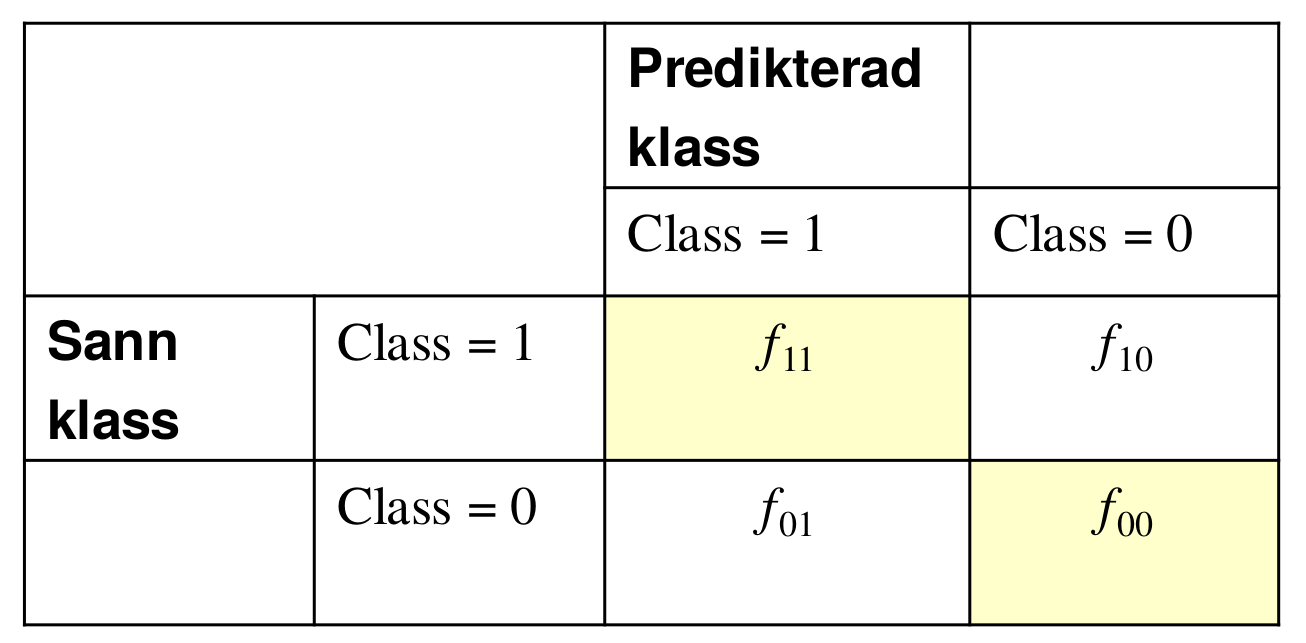
\includegraphics[width=0.7\textwidth]{figs/Screenshot at 2020-08-18 12-24-31.png}
\end{center}

\begin{itemize}
    \item Precision:
    \begin{equation*}
        \operatorname{P} = \frac{f_{11} + f_{00}}{f_{11} + f_{10} + f_{01} + f_{00}}.
    \end{equation*}
    \item Felkvot (error rate):
    \begin{equation*}
        \operatorname{E} = \frac{f_{10} + f_{01}}{f_{11} + f_{10} + f_{01} + f_{00}}.
    \end{equation*}
\end{itemize}
    
\end{frame}

\begin{frame}{Förväxlingsmatris}
    \begin{center}
        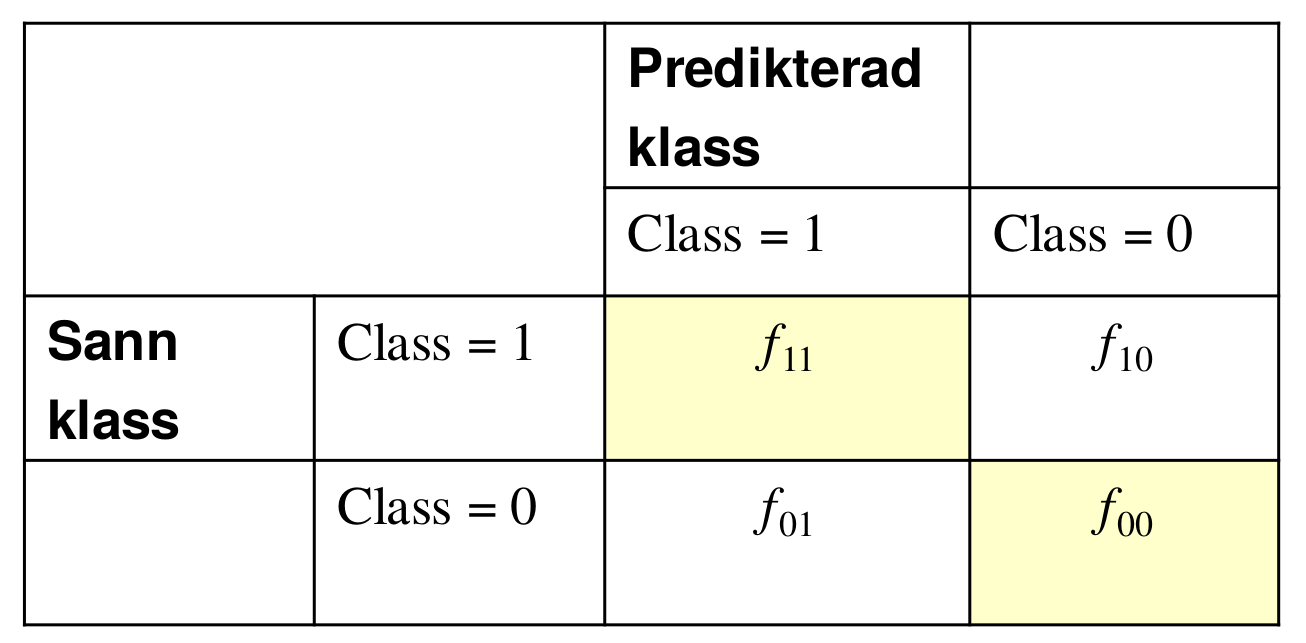
\includegraphics[width=0.7\textwidth]{figs/Screenshot at 2020-08-18 12-24-31.png}
    \end{center}
    
    \begin{itemize}
        \item Sensitivitet (recall, hit rate, true positive rate):
        \begin{equation*}
            \operatorname{TPR} = \frac{f_{11} }{f_{11} + f_{10}}.
        \end{equation*}
        \item Specifitet (selectivity, true negative rate):
        \begin{equation*}
            \operatorname{TNR} = \frac{f_{00}}{f_{00} + f_{01}}.
        \end{equation*}
    \end{itemize}
        
\end{frame}

\begin{frame}{F-score}
    
    \begin{itemize}
        \item F-score är ett mått av träffsäkerhet baserat på precision och sensitivitet.
        \begin{equation*}
            F_{\beta} = (1 + \beta^2) \frac{\operatorname{P} \cdot \operatorname{TPR}}{\beta^2 \cdot \operatorname{P} + \operatorname{TPR}}
        \end{equation*}
        \item Vanligt med $\beta=1$ vilket ger (harmoniska medelvärdet)
        \begin{equation*}
            F_1 = 2 \frac{\operatorname{P} \cdot \operatorname{TPR}}{\operatorname{P} + \operatorname{TPR}}
        \end{equation*}
        \item F-score är mellan 0 och 1, högre är bättre.
        \item $\beta$ säger hur du värderar precision och sensivitet.
        \item Beräknas klassvis.
    \end{itemize}

\end{frame}

\begin{frame}{Generaliserade linjära modeller}

    Antag att data $\mathbf{y} = y_1, y_2, \ldots, y_n$ är oberoende observationer från sannolikhetsfördelning från exponentialfamiljen.

    Vi har en linjär prediktor $\mathbf{X} \beta$ samt en länkfunktion $g$ som kopplar ihop prediktorn med medelvärdet $\mu$ genom
    \begin{equation*}
        g(\mu) = \mathbf{X} \beta.
    \end{equation*}
    
    Tar "vanlig" linjär regression till andra typer av responsvariabler
    \begin{itemize}
        \item Kontinuerlig: Normal, t, gamma, log-normal
        \item Binär: Logistisk regression
        \item Nominell: Multinomiell logistisk regression
        \item Frekvensdata: Poisson regression
    \end{itemize}
\end{frame}

\begin{frame}{Generaliserade linjära modeller - Exempel}

    \myheading{Linjär regression}
    \begin{itemize}
        \item Likelihood: Normal
        \item L\"ankfunktion: identitetsfunktionen
        \item SKattas genom att minimera:
        \begin{equation*}
            \operatorname{RSS} = \sum_{i=1}^{n} \left( y_i - \beta_0 - \sum_{j=1}^{p} \beta_j x_{ij} \right)^2
        \end{equation*}
    \end{itemize}

\end{frame}

\begin{frame}{Generaliserade linjära modeller - Exempel}
    \myheading{Logistisk regression}
    \begin{itemize}
        \item Likelihood: Bernoulli ($y$ kan vara 0 eller 1, $\mathbb{P}(y = 1) = p$)
        \item L\"ankfunktion: Logit,
        \begin{equation*}
            g(\mu) = \log\left( \frac{\mu}{1-\mu} \right)
        \end{equation*}
        \item Skattas med att maximera MLE
    \end{itemize}
\end{frame}

% \begin{frame}{Generaliserade linjära modeller - Exempel}
%     \myheading{Multinominell logistisk regression}
%     \begin{itemize}
%         \item Likelihood: Kategorisk ($y$ kan ta $K$ olika värden, $\mathbb{P}(y = k) = p_k$)
%         \item L\"ankfunktion: Logit,
%         \begin{equation*}
%             g(\mu) = \log\left( \frac{\mu}{1-\mu} \right)
%         \end{equation*}
%         \item Skattas med att maximera MLE
%     \end{itemize}
% \end{frame}

\begin{frame}{Modellval för linjära regression}

    Utgå ifrån: $y$ kontinuerlig med normal likelihood.

    Vi har ett antal förklarande variabler $\mathbf{x} = (x_1, \ldots, x_p)$. Vill hitta parametrar/modell som ger minst generaliseringsfel.

    Två alternativ:
    \begin{itemize}
        \item Alternativ 1: Välj ut en delmängd av variablerna.
        \begin{itemize}
            \item Best subset, forward selection, backward selection
        \end{itemize}
        \item Alternativ 2: Behåll alla variabler men begränsa parametrarna.
        \begin{itemize}
            \item Regularisering, Ridge och Lasso.
        \end{itemize}  
    \end{itemize}
    
\end{frame}

\begin{frame}{Utvärderingsmått}
    Om vi har flera modeller, hur jämför vi dessa?

    Två alternativ:
    \begin{itemize}
        \item Indirekt skatta testfelet
        \begin{itemize}
            \item Utgå från träningsmängden
            \item Försök att minska den bias som uppstår när vi inte använder all data.
        \end{itemize}
        \item Direkt skatta testfelet
        \begin{itemize}
            \item Valideringsdata
            \item Korsvalidering
        \end{itemize}
    \end{itemize}
\end{frame}

\begin{frame}{Indirekt skatta testfelet}
    MSE på träningsdatan underskattar "riktiga" MSE värdet, kan inte användas för att välja modell.

    Idé: justera träningsfelet för att ta hänsyn till detta. 

    \begin{equation*}
        C_p = \frac{1}{n} (\operatorname{RSS} + 2 d \hat{\sigma}^2),
    \end{equation*}

    Litet $C_p$ är bäst.

    \begin{equation*}
        \text{adjusted R}^2 = 1 - \frac{\operatorname{RSS}/(n-d-1)}{\operatorname{TSS}/(n-1)},
    \end{equation*}
    där
    \begin{equation*}
        \operatorname{TSS} = \sum_{i=1}^{n}(y_i - \bar{y})^2.
    \end{equation*}

    Stort $\text{adjusted R}^2$ är bäst.
\end{frame}

\begin{frame}{Indirekt skatta testfelet}
    
    Tre andra mått AIC, BIC och HQIC är baserade på MLE skattning ev modeller.

    Låt $\log(\hat{L})$ vara log-likelihood för optimala parametervärden.

    \begin{align*}
        \operatorname{AIC} &= 2 d - 2 \log(\hat{L}) \\
        \operatorname{BIC} &= d \cdot \log(n) - 2 \log(\hat{L}) \\
        \operatorname{HQIC} &= d \cdot \log(\log(n)) - 2 \log(\hat{L}) 
    \end{align*}

    Lågt värde är bättre.

\end{frame}

\begin{frame}{Indirekt skatta testfelet}
    
    \myheading{Linjär Regression}

    \begin{align*}
        \operatorname{AIC} &= \frac{1}{n \hat{\sigma}^2} (\operatorname{RSS} + 2 d \hat{\sigma}^2) \\
        \operatorname{BIC} &= \frac{1}{n \hat{\sigma}^2} (\operatorname{RSS} + \log(n) d \hat{\sigma}^2) \\
        \operatorname{HQIC} &= \frac{1}{n \hat{\sigma}^2} (\operatorname{RSS} + \log(\log(n)) d \hat{\sigma}^2)
    \end{align*}

    För linjär regression är $C_p \propto \operatorname{AIC}$.

    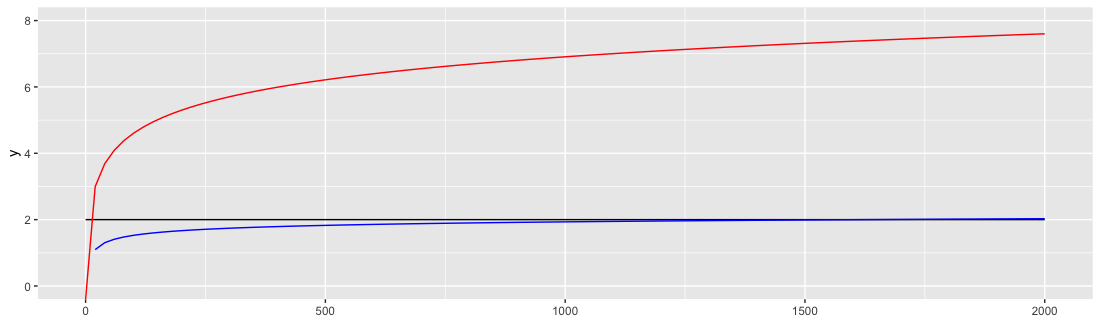
\includegraphics[width = \textwidth]{figs/logplot.png}

\end{frame}

\begin{frame}{Best subset selection}
    \begin{nscenter}
        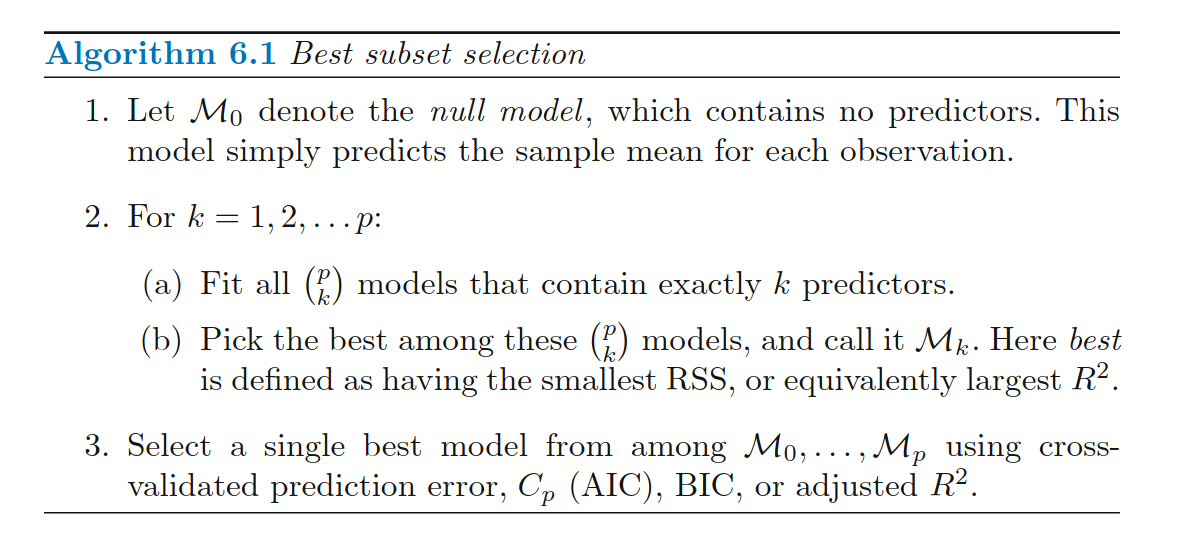
\includegraphics[width=\textwidth]{figs/best subset selection.png}
    \end{nscenter}
    Bild från kursboken "An Introduction to Statistical Learning with Applications in R".

\end{frame}

\begin{frame}{Forward selection}
    \begin{nscenter}
        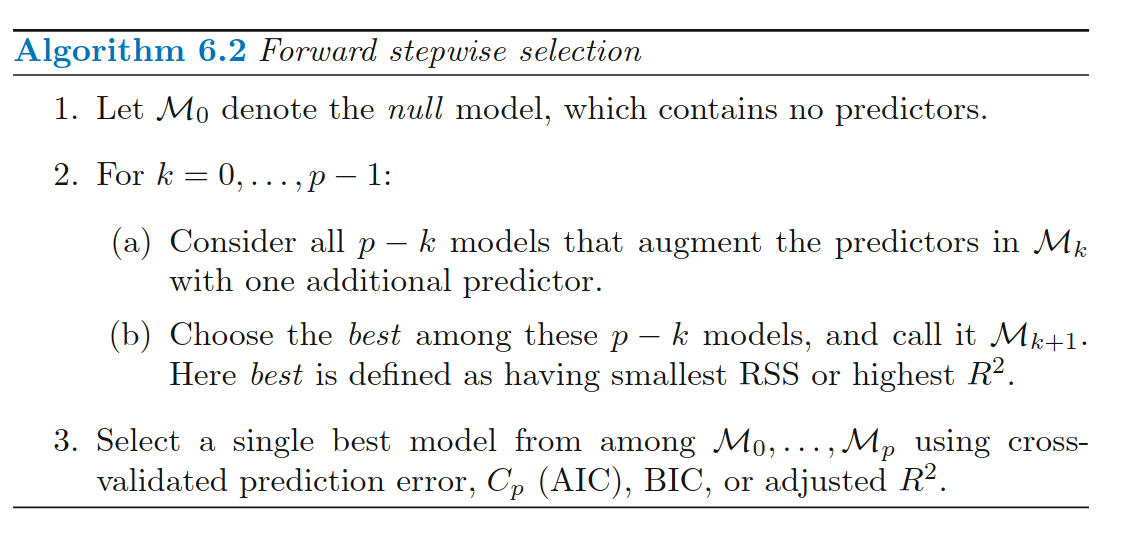
\includegraphics[width=\textwidth]{figs/Forward stepwise selection.png}
    \end{nscenter}
    Bild från kursboken "An Introduction to Statistical Learning with Applications in R".

\end{frame}

\begin{frame}{Backward selection}
    \begin{nscenter}
        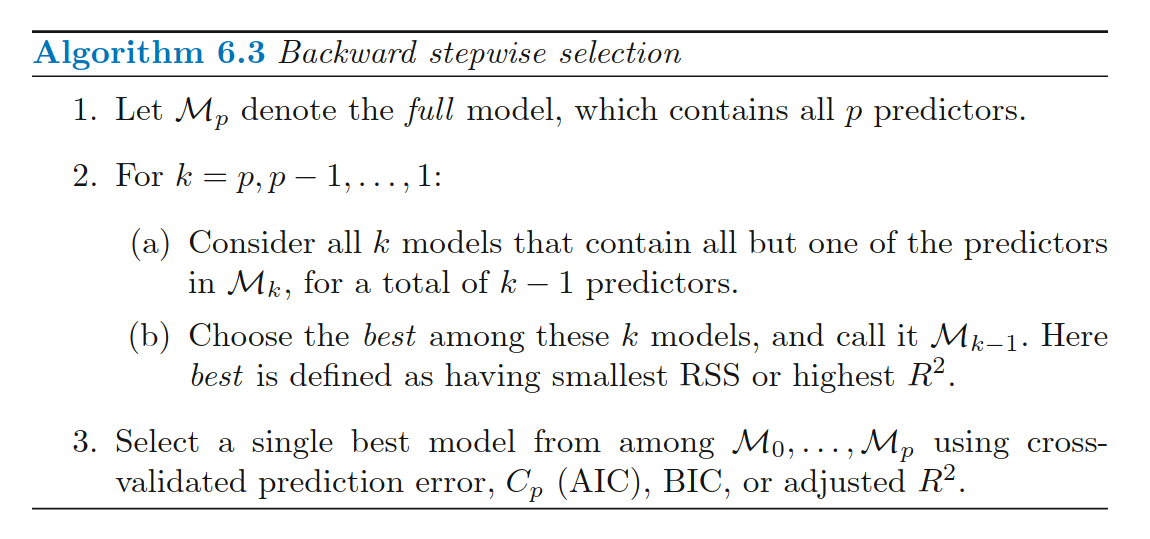
\includegraphics[width=\textwidth]{figs/Backward stepwise selection.png}
    \end{nscenter}
    Bild från kursboken "An Introduction to Statistical Learning with Applications in R".

\end{frame}

\begin{frame}{Krympning (Shrinkage)}
    
    Idé: begränsa hur stora parametrarna får vara.
    \begin{itemize}
        \item Straffa stora parametrar
        \item Ändra deras värdemängd
    \end{itemize}
    Vanligaste metoderna:
    \begin{itemize}
        \item Ridge: $l^2$-norm
        \item Lasso: $l^1$-norm
    \end{itemize}

    Kom ihåg att standardisera era förklarande variabler först innan krympning!

\end{frame}

\begin{frame}{Ridge Regression}

    I vanliga regression minimerar vi
    \begin{equation*}
        f(\beta) = \operatorname{RSS} = \sum_{i=1}^{n}\left(y_i - \beta_0 - \sum_{j=1}^{p}\beta_j x_{ij}\right)^2
    \end{equation*}
    I Ridge lägger vi till $l^2$-norm på $\beta$ vilket ger
    \begin{equation*}
        f_{\text{Ride}}(\beta) = \sum_{i=1}^{n}\left(y_i - \beta_0 - \sum_{j=1}^{p}\beta_j x_{ij}\right)^2 + \lambda \sum_{j=1}^{p} \beta_j^2, \quad \lambda \geq 0.
    \end{equation*}
    $\lambda$ är en \textbf{hyperparameter} som vi behöver sätta.

    Notera att $\beta_0$ inte påverkas.
    
\end{frame}

\begin{frame}{Ridge Regression}

    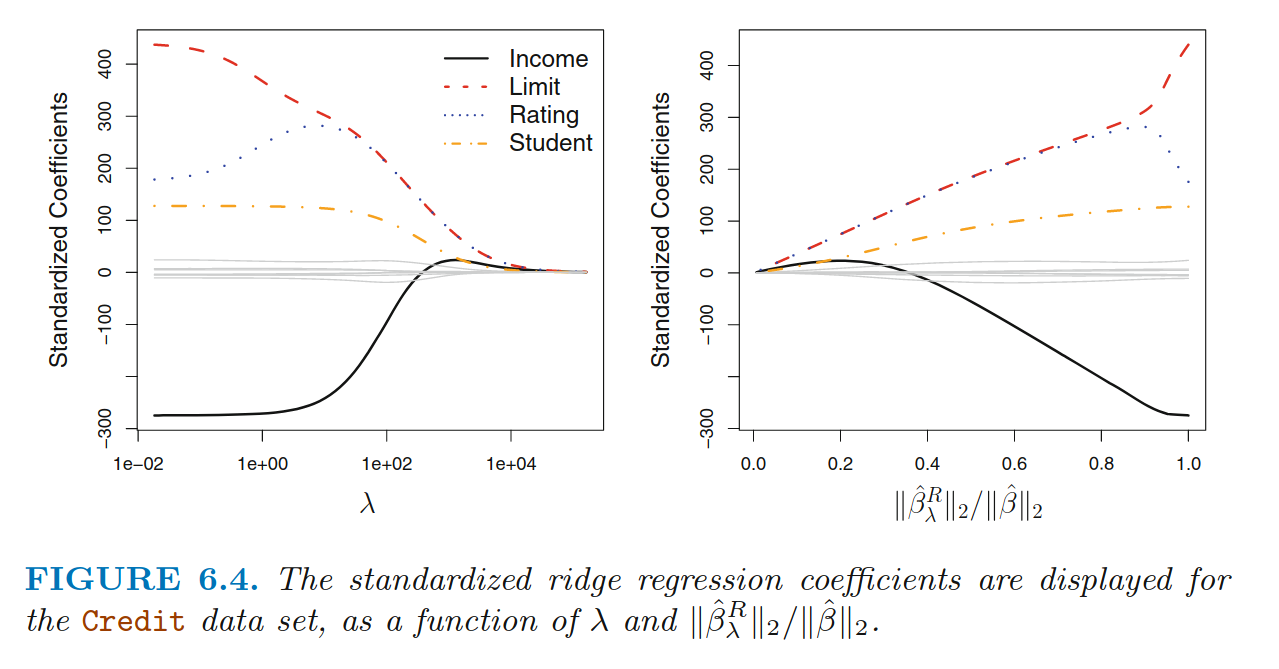
\includegraphics[width=\textwidth]{figs/standardized ridge regression coefficients.png}
    
\end{frame}

\begin{frame}{Lasso Regression}
    I vanliga regression minimerar vi
    \begin{equation*}
        f(\beta) = \operatorname{RSS} = \sum_{i=1}^{n}\left(y_i - \beta_0 - \sum_{j=1}^{p}\beta_j x_{ij}\right)^2
    \end{equation*}
    I Ridge lägger vi till $l^1$-norm på $\beta$ vilket ger
    \begin{equation*}
        f_{\text{Ride}}(\beta) = \sum_{i=1}^{n}\left(y_i - \beta_0 - \sum_{j=1}^{p}\beta_j x_{ij}\right)^2 + \lambda \sum_{j=1}^{p} |\beta_j|, \quad \lambda \geq 0.
    \end{equation*}
    $\lambda$ är en \textbf{hyperparameter} som vi behöver sätta.

    Notera att $\beta_0$ inte påverkas.
\end{frame}

\begin{frame}{Lasso Regression}
    
    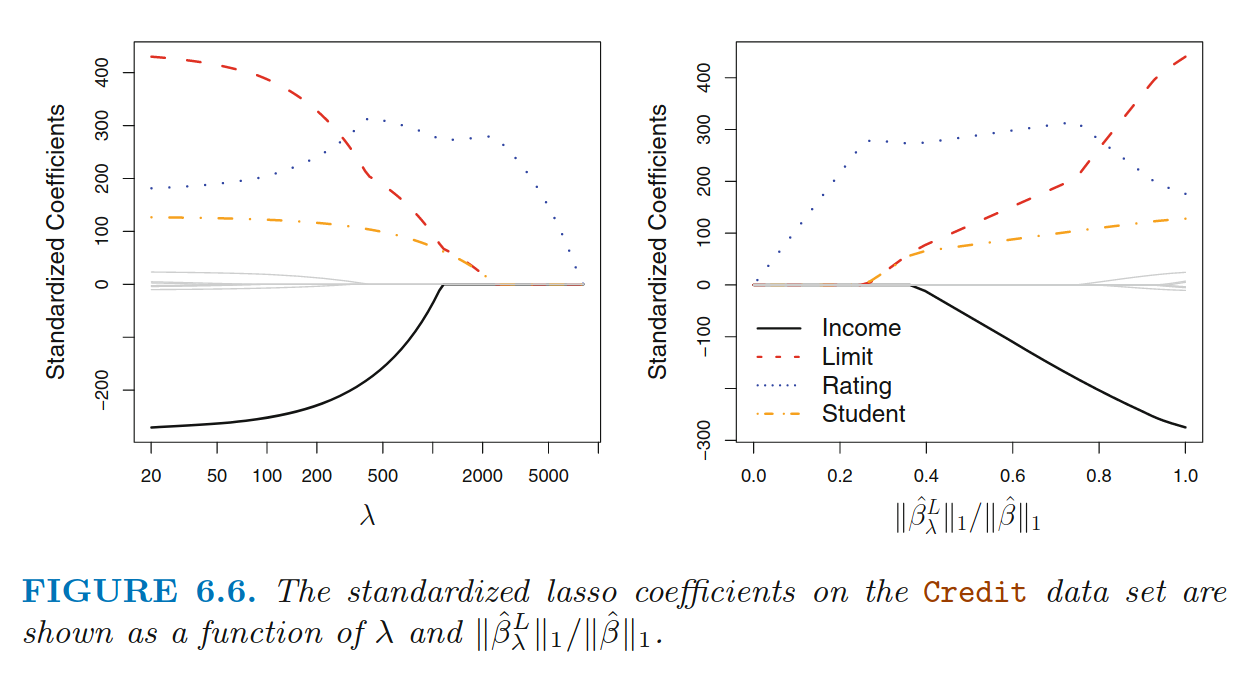
\includegraphics[width=\textwidth]{figs/standardized lasso coefficients.png}

\end{frame}

\begin{frame}{Ridge vs Lasso}
    \begin{tabular}{lll}
        & Ridge & Lasso \\ \hline
        $\lambda \to 0$ & $\hat{\beta}_{\text{Ridge}} \to \hat{\beta}_{\text{OLS}}$ & $\hat{\beta}_{\text{Lasso}} \to \hat{\beta}_{\text{OLS}}$ \\
        $\lambda \to \infty$ &  $\hat{\beta}_{\text{Ridge}} \to 0$ &  $\hat{\beta}_{\text{Lasso}} \to 0$ \\
        Norm & $l^2$-norm & $l^1$-norm \\
        Område & Hypersfär & Polytop \\
        Parametrar & Krymper och ger många små & Sätter många till 0 \\
        Korrelerade variable & Krymper alla lika mycket & Sätter en till 0
    \end{tabular}
\end{frame}

\begin{frame}{Ridge vs Lasso}

    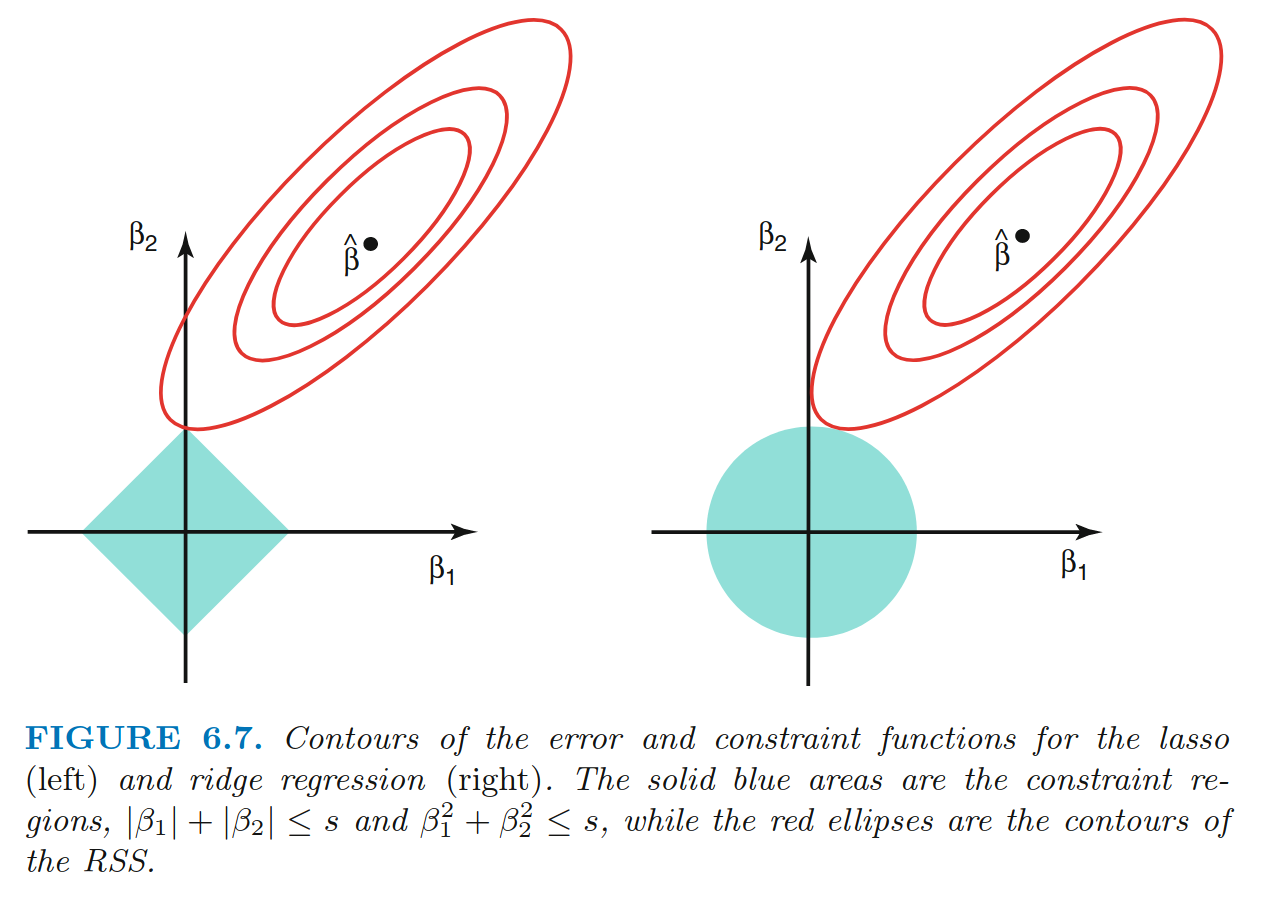
\includegraphics[width=\textwidth]{figs/Contours of the error .png}
    
\end{frame}

\begin{frame}{Ridge vs Lasso}
    
    \begin{itemize}
        \item I R, skattas enkelt med \texttt{glmnet()} eller \texttt{cv.glmnet()}.
        \item Vilken som är bäst beror på kontext.
        \item Ridge passar bra när $y$ beror på de flesta variablerna.
        \begin{itemize}
            \item Många variabler och ungefär samma effektstorlek.
        \end{itemize}
        \item Lasso passar bra när $y$ beror på bara några få variabler.
        \begin{itemize}
            \item Fåtal variabler med hög effektstorlek, resten nära 0.
        \end{itemize}
        \item Lasso kan vara lättare att tolka.
        \item Lättare att göra inference på parameterarna i Ridge.
        \item Vilken man ska välja får ofta avgöras empiriskt för specifika dataset.
        \item Finns många utökningar.
    \end{itemize}

\end{frame}

\begin{frame}{Adaptive-Lasso}
    \begin{itemize}
        \item Låt varje parameter $\beta_j$ ha sin egen vikt $w_j$
        \begin{equation*}
            f(\beta) = \sum_{i=1}^{n}\left(y_i - \beta_0 - \sum_{j=1}^{p}\beta_j x_{ij}\right)^2 + \lambda \sum_{j=1}^{p} w_j |\beta_j|, \quad \lambda \geq 0.
        \end{equation*}
        \item Välj vikter
        \begin{equation*}
            w_j = | \hat{\beta}_{j, \text{start}} |^{-\gamma}
        \end{equation*}
        \item Ofta väljs $\gamma = 1$.
        \item Behöver startvärde $\hat{\beta}_{j,\text{start}}$, kan använda OLS eller Ridge skattning.
        \item Stora startvärden ger små vikter vilket gör att parametern krymper mindre.
        \item Finns vissa teorestiska fördelar, men kräver extra skattning.
    \end{itemize}
\end{frame}

\begin{frame}{Elasticnet regression}

    \begin{itemize}
        \item Kombinerar Ridge och Lasso.
        \item Ny hyperparameter $\alpha$ för att mixa dessa,
        \begin{equation*}
            f(\beta) = \operatorname{RSS} + \lambda \left((1-\alpha) \sum_{j=1}^{p}\beta_j^2 + \alpha \sum_{j=1}^{p}|\beta_j|  \right), \qquad \lambda \geq 0,\, 0 \leq \alpha \leq 1.
        \end{equation*}
        \item $\lambda$ är likt tidigare hur mycket regularisering vi gör.
        \item $\alpha$ väljer hur mycket vikt vid Ridge respektive Lasso.
        \item Kan tvinga vissa $\beta$ till 0, men inte lika många som Lasso.
        \item Klarar av korrelerade/grupper av variabler bättre än Lasso.
        \item Nackdel är att vi har två hyperparametrar.
    \end{itemize}
    
\end{frame}


\end{document}